\documentclass{beamer}

% Required packages
\usepackage{fontspec}
\usepackage{fontawesome}
\usepackage{parskip}
\usepackage{hyperref}
\hypersetup{
  colorlinks=false,
  linkbordercolor={white}
}
\usepackage{bookmark}
\usetheme{metropolis}           

\title{AMSE - \textit{MeinBundestag}}
\date{February 3, 2020}
\author{Benjamin Fischer}
\institute{\faInstitution{}\quad{}Friedrich-Alexander Universität Erlangen-Nürnberg}
\newcounter{index}
\stepcounter{index}


\begin{document}
  \maketitle

  \begin{frame}[plain]{MeinBundestag}
    \begin{itemize}
      \item[\faEnvelope]\quad
      \texttt{benjamin.f.fischer@fau.de}
      \item[\faGithub]\quad
      \href{https://github.com/fischerbenjamin/meinbundestag}{\texttt{fischerbenjamin/meinbundestag}}
      \item[\faCopyright]\quad
      \texttt{MIT License}
      \item[\faCogs]\quad
      \texttt{development, not standalone}
    \end{itemize} 
  \end{frame}

  \section{Motivation}
  \begin{frame}[plain]{Motivation}
    \begin{itemize}
      \item[\faInfoCircle]\quad
      \textbf{Idea}
      \begin{itemize}
        \item Informative application about the German parliament
        \item Running on a mobile device (Android/iOS)
      \end{itemize}
      \item[\faBars]\quad
      \textbf{Features}
      \begin{itemize}
        \item Search for a certain deputy or location
        \item Receive general information about the deputy
        \item Read the speeches held by the deputy in the parliament
      \end{itemize}
      \item[\faHeart]\quad
      \textbf{Goal}
      \begin{itemize}
        \item Provide information the user otherwise would not look for
        \item Increase political interest
      \end{itemize}
    \end{itemize}
  \end{frame}

  \section{Demo}

  \section{OpenData}
  \begin{frame}[plain]{OpenData}
    \textbf{\faAt}\quad\textbf{www.bundestag.de/services/opendata}
    \begin{itemize}
      \item Protocols of the parliament given as \texttt{.xml} files
      \item Providing an additional \texttt{.dtd} file for processing
      \item Current election period (since 2017)
      \item Files are updated according to the session schedule
    \end{itemize}
    \textbf{\faExclamationTriangle}\quad\textbf{Problems}
    \begin{itemize}
      \item Only the latest five protocols are included in the table
      \item Loading other protocols requires the user clicking on buttons
    \end{itemize}  
  \end{frame}

  \begin{frame}[plain]{OpenData}
    \textbf{\faAt}\quad\textbf{www.abgeordnetenwatch.de/api/parliament/bundestag}
    \begin{itemize}
      \item Information about each deputy of the parliament
      \item Votings, secondary activities, etc.
      \item List of all deputies: /deputies.json
      \item Profile of a single deputy: profile/\textit{\{deputy\}}/profile.json
    \end{itemize}
  \end{frame}

  \section{Technology}
  \begin{frame}[plain]{Technology}
    \begin{center}
      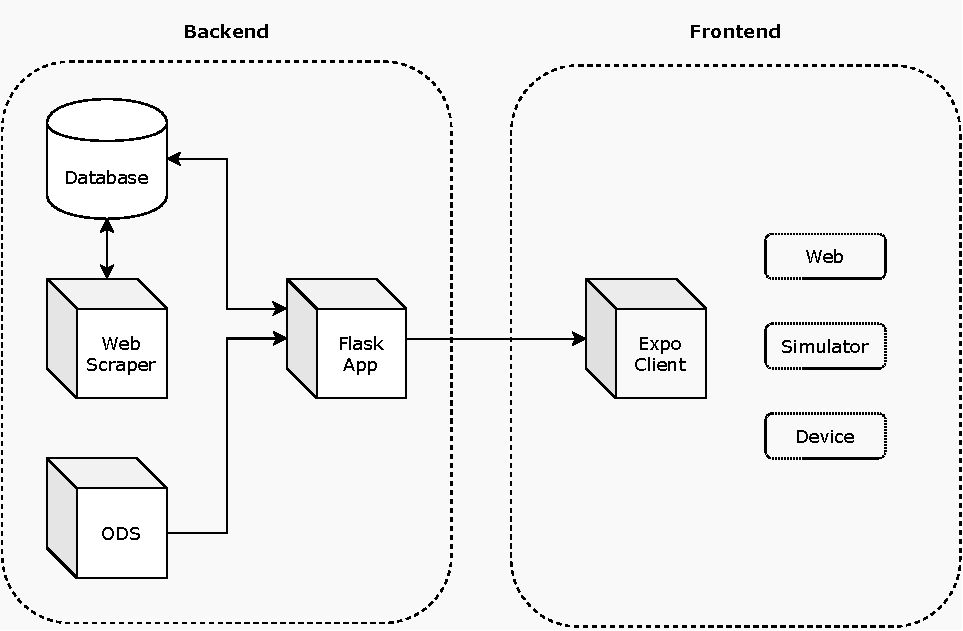
\includegraphics[width=0.99\textwidth]{fig/technology_overview.pdf}
    \end{center}
  \end{frame}

  \begin{frame}[plain]{Technology}
    \textbf{\faDesktop}\quad\textbf{Frontend}
    \begin{itemize}
      \item React Native\textsuperscript{\hyperlink{link-react-native}{\arabic{index}}} application
      \stepcounter{index}
      \item Usage of Expo\textsuperscript{\hyperlink{link-expo}{\arabic{index}}} for easier development
      \stepcounter{index}
      \item Minimalistic, platform-independent code
    \end{itemize}
    \textbf{\faServer}\quad\textbf{Backend}
    \begin{itemize}
      \item Python Flask\textsuperscript{\hyperlink{link-flask}{\arabic{index}}} application provides the API
      \stepcounter{index}
      \item Selenium\textsuperscript{\hyperlink{link-selenium}{\arabic{index}}} web scraper searching for new protocols
      \stepcounter{index}
      \item MongoDB\textsuperscript{\hyperlink{link-mongodb}{\arabic{index}}} database persists processed protocol data
      \stepcounter{index}
      \item Database and API are running in seperate Docker\textsuperscript{\hyperlink{link-docker}{\arabic{index}}} container
    \end{itemize}
  \end{frame}

  \section{ODS}
  \begin{frame}[plain]{ODS}
    \textbf{Specific}
    \begin{itemize}
      \item The ODS is used for providing the list of all deputies
      \item Not applicable for protocol data (obviously)
      \item Providing profile data would require supporting placeholders
    \end{itemize}
    \textbf{General}
    \begin{itemize}
      \item Idea is cool, especially when working in multiple small projects
      \item Easy to setup, at least for Linux systems
      \item TODO: naming storage links and duration of storage
      \item Supporting query parameters and placeholders would be great! 
    \end{itemize} 
  \end{frame}

  \begin{frame}[plain]{Links}
    \begin{itemize}
      \item[] \label{link-react-native}\href{https://facebook.github.io/react-native}{\texttt{https://facebook.github.io/react-native}}
      \item[] \label{link-expo}\href{https://expo.io/}{\texttt{https://expo.io/}}
      \item[] \label{link-flask}\href{https://www.fullstackpython.com/flask.html}{\texttt{https://www.fullstackpython.com/flask.html}}
      \item[] \label{link-selenium}\href{https://selenium-python.readthedocs.io/}{\texttt{https://selenium-python.readthedocs.io/}}
      \item[] \label{link-mongodb}\href{https://www.mongodb.com/}{\texttt{https://www.mongodb.com/}}
      \item[] \label{link-mongodb}\href{https://www.docker.com/}{\texttt{https://www.docker.com/}}
    \end{itemize}
  \end{frame}



  \begin{frame}[plain]{}
    \centering
    \Large \textbf{Thank you for your attention!}\\
    \vspace{2em}
    \Large \textbf{Questions?}
  \end{frame}



\end{document}